%%%%%%%%%%%%%%%%%%%%%%%%%%%%%%%%%%%%%%%%%%%%%%%%%%%%%%%%%%%%%%%%%%%%%%%%%%%%%%%%
% AMS Beamer series / Bologna FC / Template
% Andrea Omicini
% Alma Mater Studiorum - Università di Bologna
% mailto:andrea.omicini@unibo.it
%%%%%%%%%%%%%%%%%%%%%%%%%%%%%%%%%%%%%%%%%%%%%%%%%%%%%%%%%%%%%%%%%%%%%%%%%%%%%%%%
%\documentclass[handout]{beamer}\mode<handout>{\usetheme{default}}
%
\documentclass[presentation, 9pt, aspectratio=169]{beamer}\mode<presentation>{\usetheme{AMSBolognaFC}}
%\documentclass[handout]{beamer}\mode<handout>{\usetheme{AMSBolognaFC}}
%%%%%%%%%%%%%%%%%%%%%%%%%%%%%%%%%%%%%%%%%%%%%%%%%%%%%%%%%%%%%%%%%%%%%%%%%%%%%%%%
\usepackage[T1]{fontenc}
\usepackage{wasysym}
\usepackage{amsmath,blkarray}
\usepackage{soul}
\usepackage{centernot}
\usepackage{fontawesome}
\usepackage{fancyvrb}
\usepackage{hyperref}
\usepackage{multicol}
\usepackage[ddmmyyyy]{datetime}
\renewcommand{\dateseparator}{}
%\renewcommand{\thefootnote}{\fnsymbol{footnote}}
\newcommand{\version}{1}

\usepackage[
%	backend=biber,
	backend=bibtex,
%	citestyle=authoryear-icomp,
%	maxcitenames=1,
	bibstyle=numeric,
	style=ieee]{biblatex}

	\makeatletter

\addbibresource{biblio.bib}


\newcommand\extrafootertext[1]{%
    \bgroup
    \renewcommand\thefootnote{\fnsymbol{footnote}}%
    \renewcommand\thempfootnote{\fnsymbol{mpfootnote}}%
    \footnotetext[0]{#1}%
    \egroup
}

\newcommand{\citeinslide}[1]{\cite{#1}\extrafootertext{\scriptsize\cite{#1} \fullcite{#1}}}


%%%%%%%%%%%%%%%%%%%%%%%%%%%%%%%%%%%%%%%%%%%%%%%%%%%%%%%%%%%%%%%%%%%%%%%%%%%%%%%%
\title[Activities Summary]
{Activities Summary @ Common-Wears}
%
%
\author[\sspeaker{Aguzzi}]
{\speaker{Gianluca Aguzzi} \href{mailto:gianluca.aguzzi@unibo.it}{gianluca.aguzzi@unibo.it} \\
}
%
\institute[DISI, Univ.\ Bologna]
{%Dipartimento di Informatica -- Scienza e Ingegneria (DISI)\\
\textsc{Alma Mater Studiorum} -- Universit{\`a} di Bologna \\[0.1cm]
\textbf{Talk @} \bold{Common Wears}\\[0.15cm]
}
%
\renewcommand{\dateseparator}{/}
\date[\today]{\today}
%
\AtBeginSubsection[]
{
  \begin{frame}
  \frametitle{Contents}
  \tableofcontents[currentsubsection, 
	sectionstyle=show/shaded, 
	subsectionstyle=show/shaded]
  \end{frame}
}
\AtBeginSection[]
{
  \begin{frame}
  \frametitle{Contents}
  \tableofcontents[currentsubsection, 
	sectionstyle=show/shaded, 
	subsectionstyle=show/shaded]
  \end{frame}
}
%%%%%%%%%%%%%%%%%%%%%%%%%%%%%%%%%%%%%%%%%%%%%%%%%%%%%%%%%%%%%%%%%%%%%%%%%%%%%%%%


\newcommand{\hsplit}[2]{
\begin{minipage}{0.48\textwidth}
#1
\end{minipage}
\hfill
\begin{minipage}{0.48\textwidth}
#2
\end{minipage}
}
\newcommand{\hsplits}[4]{
\begin{minipage}{#1\textwidth}
#3
\end{minipage}
\hfill
\begin{minipage}{#2\textwidth}
#4
\end{minipage}
}

\newcommand{\lbl}[1]{\textbf{\textcolor{gray!90!white}{#1}}}
\newcommand{\enf}[1]{{\textcolor{red}{#1}}}
\newcommand{\bo}[1]{\textbf{#1}}

\newcommand{\imgh}[2]{
\begin{figure}
\centering
\includegraphics[width=#1\textwidth]{img/#2}
\end{figure}
}
\newcommand{\imgv}[2]{
\begin{figure}
\centering
\includegraphics[height=#1\textheight]{img/#2}
\end{figure}
}


\newcommand{\question}[1]{\textcolor{darkgray}{\emph{\bo{#1}}}}
\newcommand{\refslide}[1]{Slide~\ref{#1}}

\begin{document}
\frame{\titlepage}
%===============================================================================

\section{Overview}
\begin{frame}[fragile]{Activities Overview}
	\begin{figure}
		\centering
		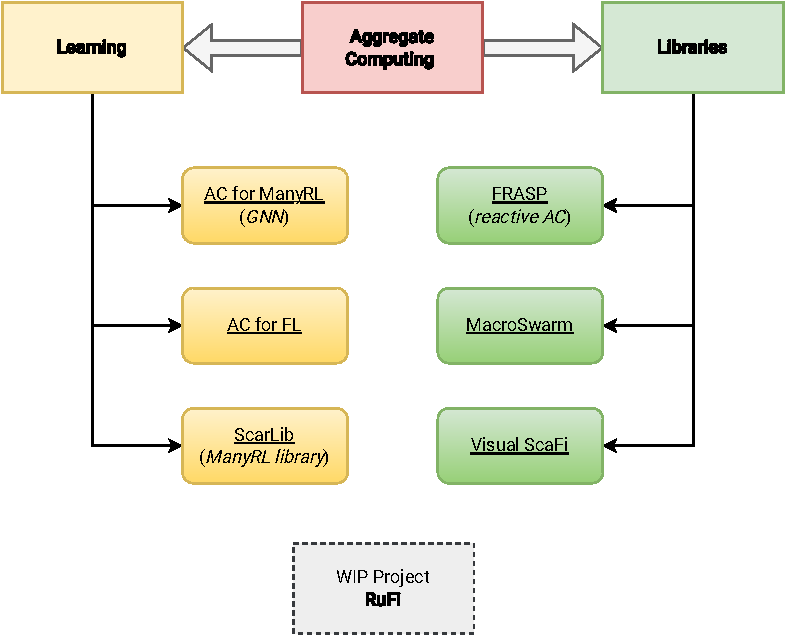
\includegraphics[width=0.55\textwidth]{img/activities-overview.drawio}
	\end{figure}
\end{frame}
\section{Learning}
\begin{frame}{Aggregate Computing for many-agent reinforcement learning: \bold{Field-informed RL}}
	\begin{alertblock}{ManyRL: pragmatic definition}
		Many-agent reinforcement learning is a framework for \emph{learning} in multi-agent systems composed by a \bold{large number} of agents (hundreds/thousands).
		
	\end{alertblock}
	\begin{exampleblock}{Common wears POV}	
		The community can be composed of a large number of agents \faArrowRight \, we need a \bold{scalable} solution.
	\end{exampleblock}
	\begin{exampleblock}{State-of-the-art solutions}
		\begin{itemize}
			\item Centralised training and decentralized execution: standard training paradigm
			\item Mean-field approximation: agents are independent and identical \faArrowRight \, mean-field reinforcement learning
			\item Our approach: \emph{Field-informed RL}
		\end{itemize}
	\end{exampleblock}
\end{frame}
\begin{frame}{Field-informed RL}
	\begin{figure}
		\centering
		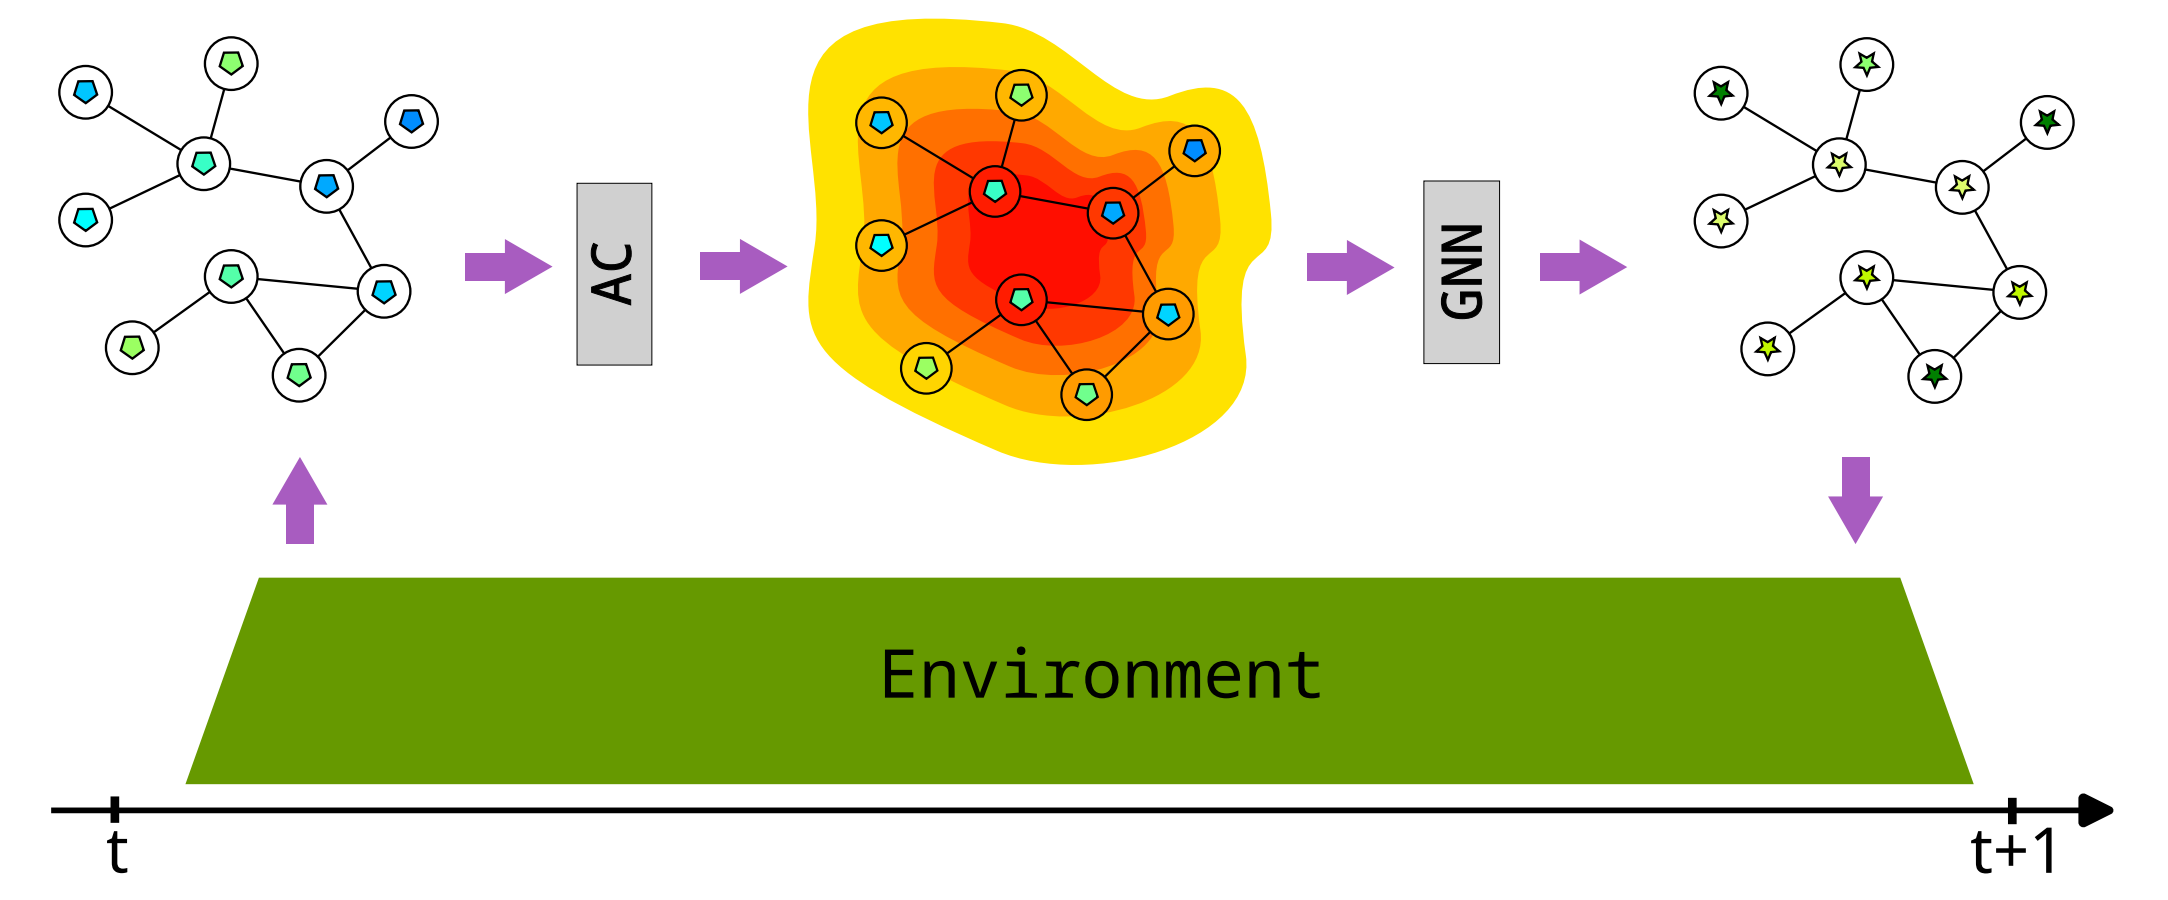
\includegraphics[width=0.6\textwidth]{img/field-informed-structure}
	\end{figure}
	\begin{figure}
		\centering
		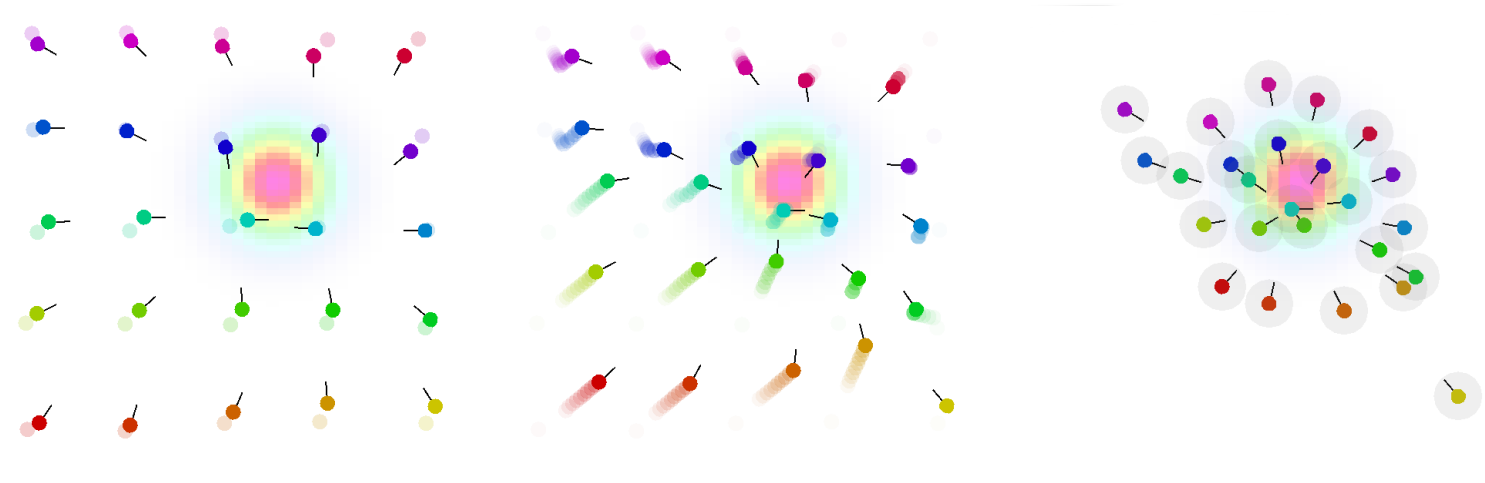
\includegraphics[width=0.6\textwidth]{img/field-informed}
	\end{figure}
\end{frame}
\begin{frame}{Field-Informed RL}
	\begin{exampleblock}{Planned activities}
		\begin{itemize}
			\item \emph{Extensive} evaluation in real-case scenarios (testbeds for common-wears???)
			\item In-depth analysis of the \emph{scalability} of the approach (i.e., how many agents can be supported?)
			\item Learning with few agents and \emph{generalization} to many agents
			\item Decentralised training (and possibly online?)
		\end{itemize}
	\end{exampleblock}
\end{frame}
\begin{frame}{Aggregate Computing for Federated Learning}
	\begin{alertblock}{Pratical definition}
		Training of \bold{decentralized} models on \bold{local} data, enhancing privacy by sharing only model updates or by sharing only the model parameters.
	\end{alertblock}
	\begin{exampleblock}{Common-wears POV}
		The sensor data can be \bold{private} and it cannot be shared (i.e., healthcare data).
	\end{exampleblock}
	\begin{exampleblock}{Aggregate computing vision: \emph{``fluid''} federated learning}
		Use aggregate computing to \emph{fluidify} the federated learning process, supporting:
		\begin{itemize}
			\item peer-to-peer topology (i.e., no central server)
			\item central-based topology (i.e., central server)
			\item hybrid topology (i.e., central server + peer-to-peer)
			\item different area of interest (i.e., different models for different areas) \faArrowRight \, \emph{space fluid}?
		\end{itemize}
	\end{exampleblock}
\end{frame}

\begin{frame}{Tool for many-agent reinforcement learning: \bold{ScaRLib}}
	\begin{alertblock}{Why?}
		Many-agent reinforcement learning is a \bold{complex} task, we need a \bold{tool} to simplify the development of RL algorithms.
	\end{alertblock}
	\begin{exampleblock}{State-of-the-art solutions}
		\begin{itemize}
			\item \emph{Ray}: a distributed execution framework for reinforcement learning
			\begin{itemize}
				\item Do not scale with the number of agents
			\end{itemize} 
			\item \emph{PettingZoo}: a Python library for multi-agent reinforcement learning simulations
			\begin{itemize}
				\item Do not consider a very large number of agents and \emph{spatial} scenarios
			\end{itemize}
		\end{itemize}
	\end{exampleblock}
	\begin{exampleblock}{Common-wears POV}
		Simplify and homogenize the development of RL algorithms in common-wears scenarios \faArrowRight \, \bold{ScaRLib}
	\end{exampleblock}
\end{frame}
\begin{frame}{ScaRLib}
 A scala framework designed to support the development of many-agent reinforcement learning systems in JVM-based environments
\vspace{0.5cm}

 \hsplit{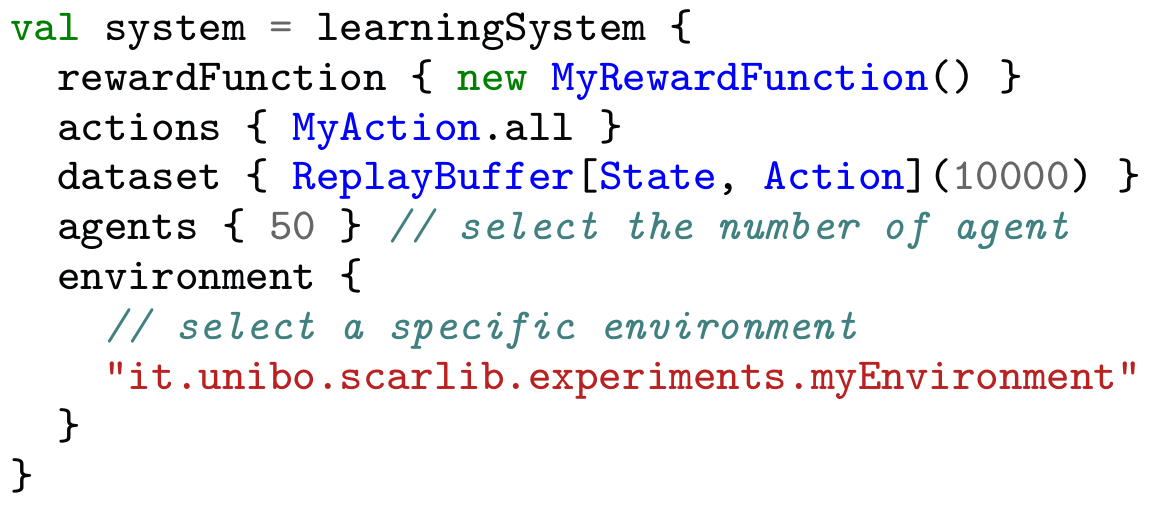
\includegraphics[width=\textwidth]{img/dsl-example}}{
	\begin{itemize}
		\item Environment-agnostic and Neural Network-agnostic API
		\item Flexible and extensible architecture for supporting different RL algorithms/training
		mode
		\item Type-safe DSL for RL algorithms configuration
		\item Special issues extension: improved documentation and example
		\item Feel free to contribute! :)
	\end{itemize}
 }
\end{frame}
\section{Libraries/API}
\begin{frame}{Reactive extension for Aggregate Computing: FRASP}
	\begin{alertblock}{Functional Reactive Programming}
		A programming paradigm for \emph{reactive} programming based on the concept of \emph{reactive values} and \emph{reactive computations}, i.e., the computation is \emph{automatically} updated when the value of a reactive value changes.
	\end{alertblock}
	\begin{exampleblock}{Common-wears POV}
		We want a pragmatic way to express spatio-temporal behavior evolution without sacrificing resource efficiency (e.g., battery, bandwidth, etc.).
	\end{exampleblock}
	\begin{exampleblock}{FRASP}
		Functional Reactive Approach to Self-organisation Programming
		\begin{itemize}
			\item designed by interpreting the aggregate programming model by a (distributed) functional
			reactive programming (FRP) perspective
			\item implemented as a Scala DSL using Sodium FRP library
		\end{itemize}
	\end{exampleblock}
\end{frame}
\begin{frame}{FRASP: Idea}
\begin{figure}
	\centering
	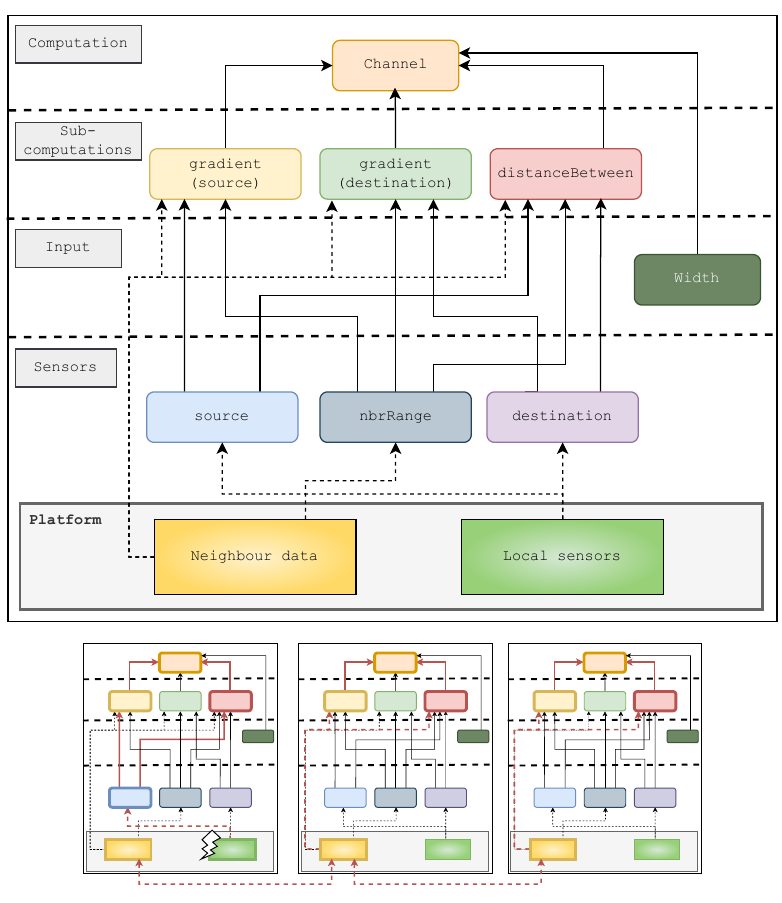
\includegraphics[width=0.4\textwidth]{img/idea}
\end{figure}
\end{frame}
\begin{frame}{FRASP: Idea}
	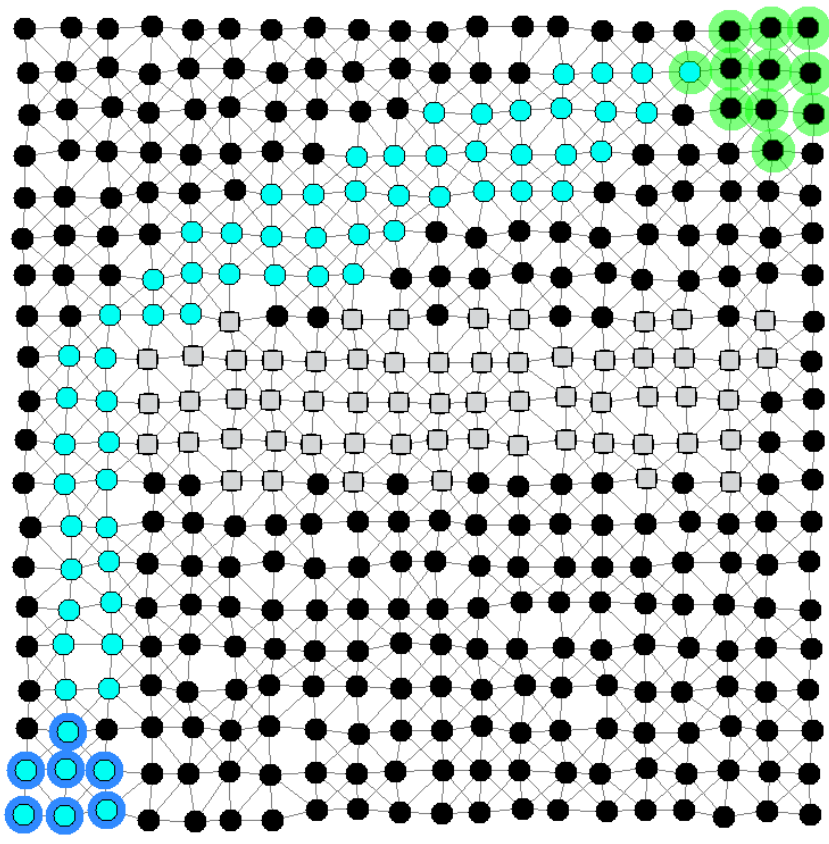
\includegraphics[width=0.24\textwidth]{img/start.png}
	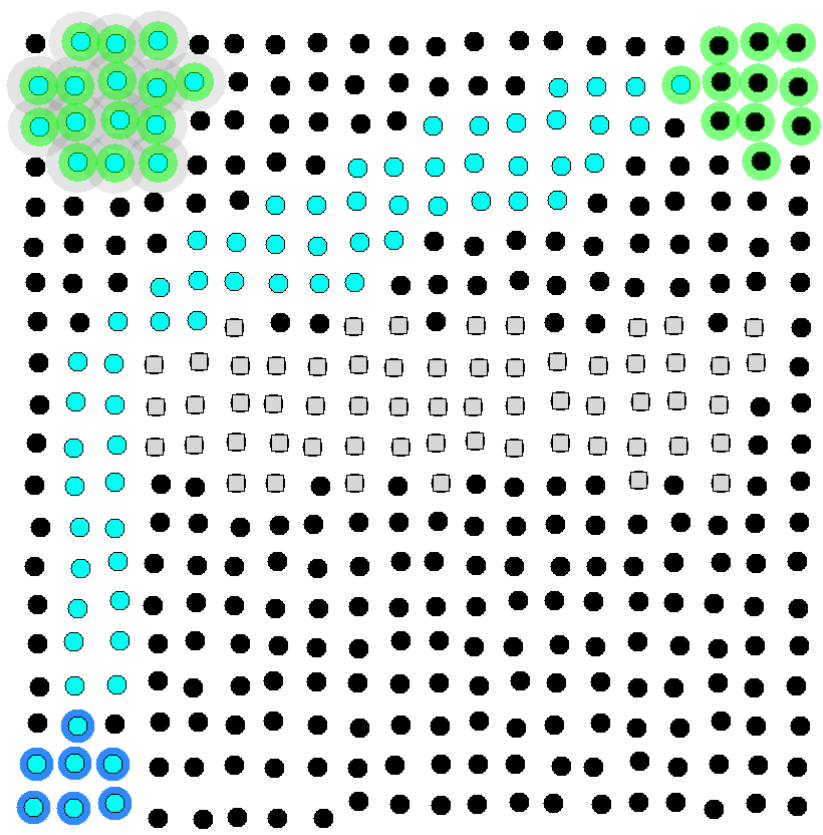
\includegraphics[width=0.24\textwidth]{img/middle.png}
	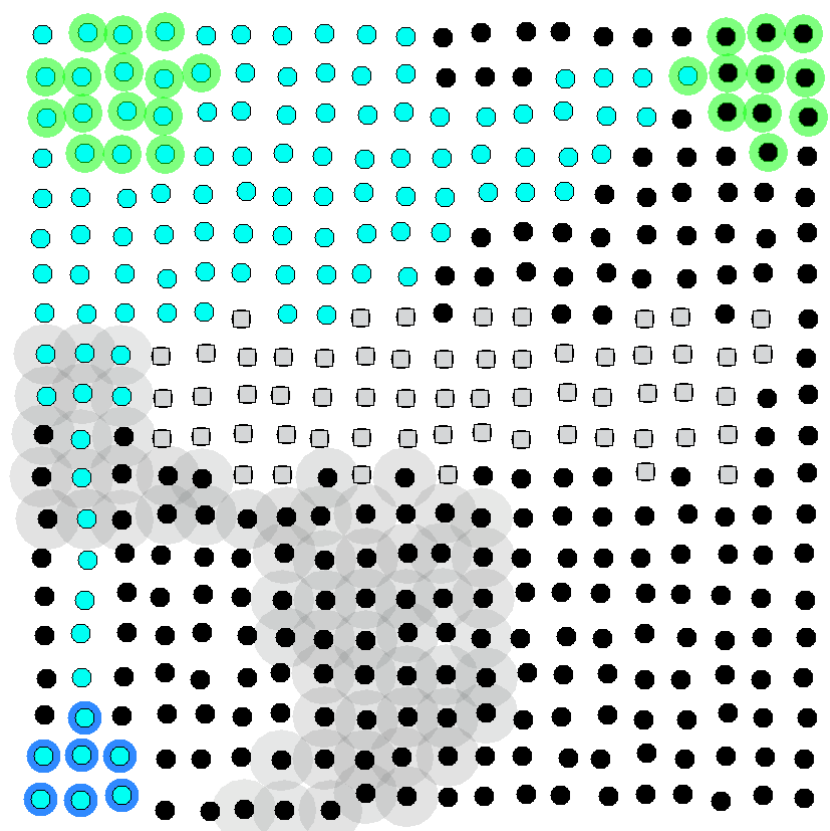
\includegraphics[width=0.24\textwidth]{img/middle-2.png}
	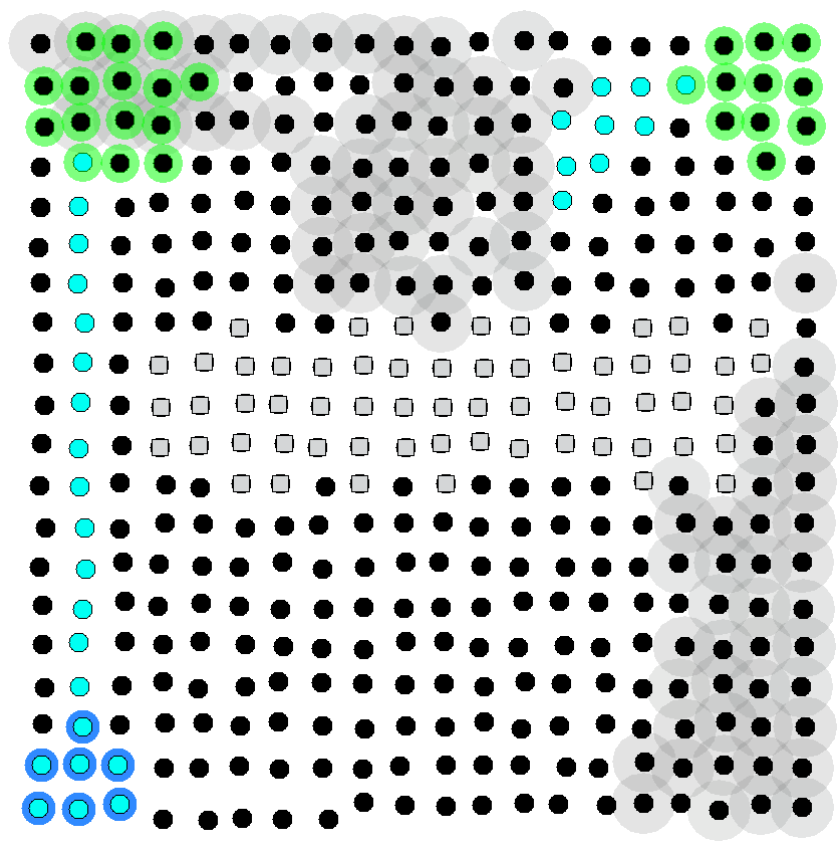
\includegraphics[width=0.24\textwidth]{img/end.png}
\end{frame}
\begin{frame}{FRASP: works in progress}
	\begin{exampleblock}
		
	\begin{itemize}
		\item Linear temporal logic for evaluation of spatiotemporal properties
		\item Support the standard library of ScaFi
		\item Kotlin implementation
		\item Middleware for executing FRASP on devices
	\end{itemize}
	\end{exampleblock}
\end{frame}
\begin{frame}{API for Swarm behaviours: MacroSwarm}

\end{frame}
\begin{frame}{Simplify the development of aggregate script: \bold{Visual ScaFi}}
	\begin{alertblock}{Visual programming}
		A programming paradigm that allows to create programs by manipulating elements graphically rather than by specifying them textually.		
	\end{alertblock}
	\begin{exampleblock}{Common-wears POV}
		We want a pragmatic way to express collective scripts without sacrificing \emph{readability} and \emph{usability}.
	\end{exampleblock}
	\begin{exampleblock}{Visual ScaFi}
		\begin{itemize}
			\item A visual programming language for aggregate computing
			\item It is based on blockly (a visual programming language developed by Google)
			\item It translates visual scripts into aggregate computing scripts (ScaFi)		
		\end{itemize}
	\end{exampleblock}
\end{frame}
\begin{frame}{Visual ScaFi WIP}
\begin{figure}
	\centering
	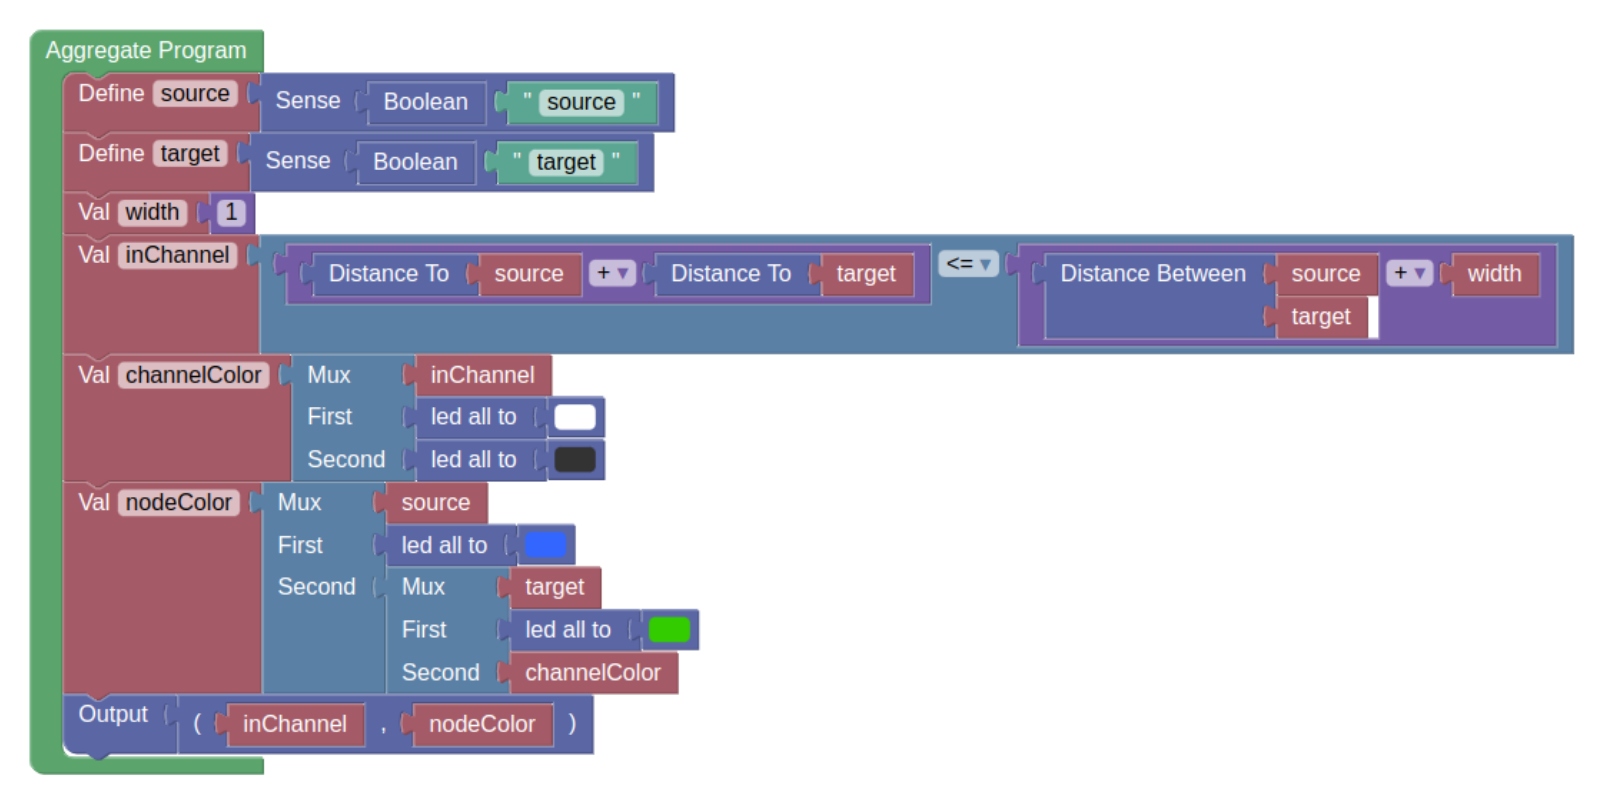
\includegraphics[width=0.8\textwidth]{img/example}
\end{figure}
\end{frame}
\section{Preliminary works in progress}
\begin{frame}{RuFi: Rust Field}
\begin{alertblock}{Common-wears POV}
	\begin{itemize}
		\item the community can be composed of low-power devices \faArrowRight \, we need a \bold{lightweight} solution.
		\item interoperability is a key aspect \faArrowRight \, we need a \bold{standard} solution.
	\end{itemize}
\end{alertblock}
\end{frame}
\section{}

%===============================================================================

%/////////
\frame{\titlepage}
%/////////

%===============================================================================
\section*{\refname}
%===============================================================================

%%%%
\setbeamertemplate{page number in head/foot}{}
%/////////


\begin{frame}[allowframebreaks]{References}
\def\bibfont{\footnotesize}
\printbibliography
\end{frame}

%%%%%%%%%%%%%%%%%%%%%%%%%%%%%%%%%%%%%%%%%%%%%%%%%%%%%%%%%%%%%%%%%%%%%%%%%%%%%%%%
\end{document}
%%%%%%%%%%%%%%%%%%%%%%%%%%%%%%%%%%%%%%%%%%%%%%%%%%%%%%%%%%%%%%%%%%%%%%%%%%%%%%%%
